\subsection{Operating Regimes and Two-Budget Maps}\label{sec:unified_maps}
\begin{figure*}[t]
\centering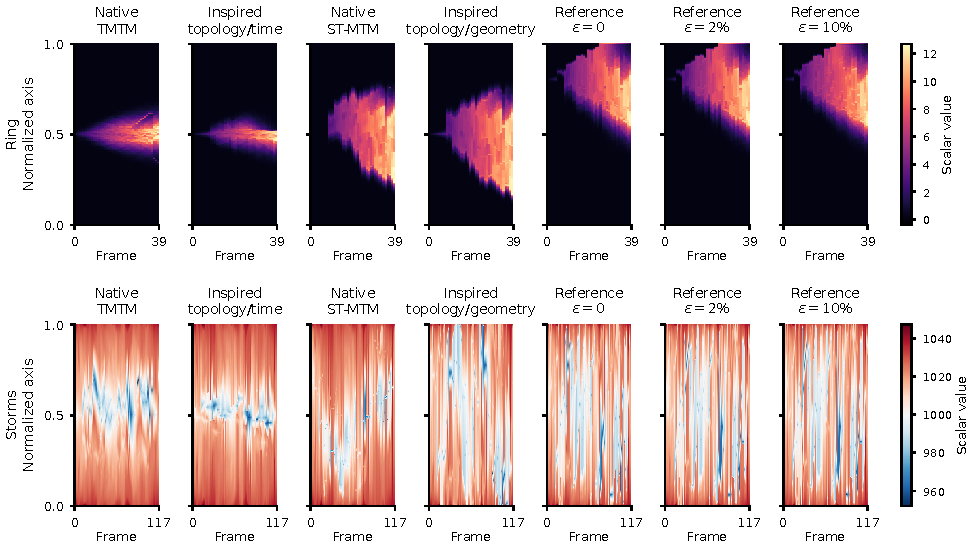
\includegraphics[width=\linewidth]{figures/Fig16.pdf}
\caption{Native methods and operating regimes of one model on Ring (top) and Storms (bottom). Within each row all columns use the same fields, time steps and scalar colours; the colour range includes corrected barrier values, which are constructed values rather than source observations. Columns 2, 4 and 5--7 share interval widths, canvas, QP and renderer; only the controls change. Native methods use their own layouts and scalar filling. All display axes are normalized to $[0,1]$; one global native reflection follows the similarity fit, with no per-frame warping. The topology/time and topology/geometry columns express inspired design principles, not native-output equality. All reference columns use $B=\infty$ and vary the true topology allowance.}\label{fig:unified_regimes}
\end{figure*}

\begin{figure*}[t]
\centering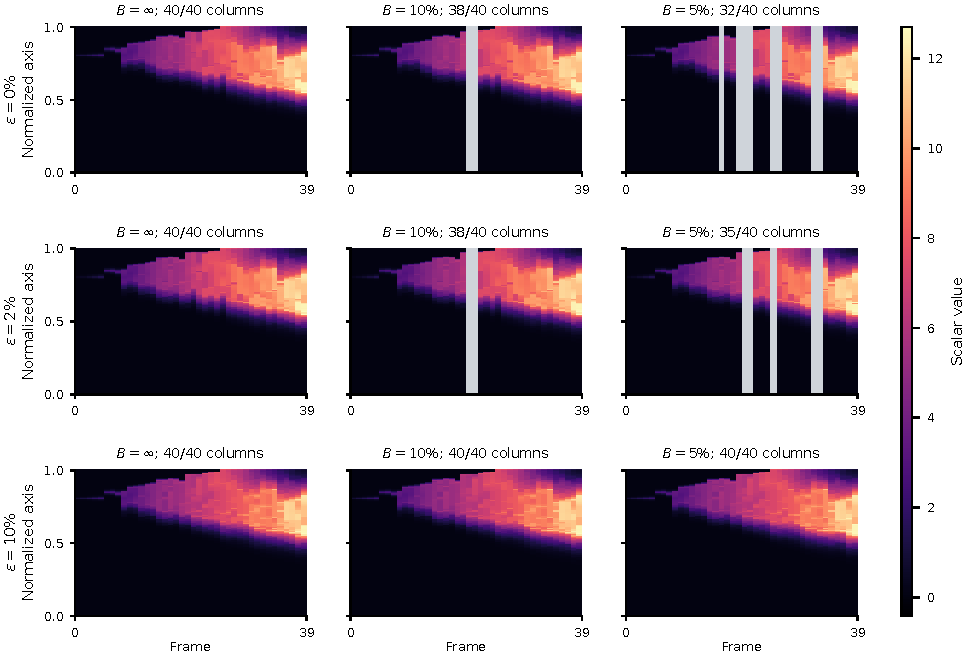
\includegraphics[width=\linewidth]{figures/Fig17.pdf}
\caption{Ring maps across topology allowances (rows) and reference-position caps (columns), using the same reference-guided objective, candidate pool and scalar renderer. Position allowances are fractions of the common canvas; topology allowances are fractions of the fixed scalar range. Gray columns denote frames for which no candidate meets both budgets, not zero scalar values. A history restarts after such a missing frame. Counts report witnessed feasible columns, rather than full-space feasibility on candidate-only frames. Finite maps include measured strict-extremum clearance and anchor rounding, which are separate from the continuous constraints.}\label{fig:unified_budget_grid}
\end{figure*}

The operating-regime views expose the difference between a topology-preserving temporal emphasis, a relative-distance emphasis, and an absolute reference target. They also show why output resemblance must be measured rather than inferred from the name of a regime. The native methods allocate widths and arrange internal samples differently. The common-model columns deliberately retain one representation so that changes can be attributed to the declared controls. The two-budget matrix additionally makes incompatible requests visible as missing witnesses instead of silently widening a tolerance.
